\chapter{Theory}
\section{X-ray photoelectron spectroscopy (XPS)}

\Acf{XPS} utilizes the ejection of electrons from a bound state to the continuum by photon excitation, called the photoelectric effect.\autocite{Hertz1887, Einstein1905} The photon energy ($E_\mathrm{\gamma}=h\nu$) of x-rays is similar to the \acl{BE} ($E_\mathrm{B}$) of deep core electrons and are therefore used for the excitation. The experiments for this work were performed with soft x-rays with an energy between 100~~~2100~\si{\eV}. For each core-level, $E_\mathrm{\gamma}$ is chosen to be slightly higher than $E_\mathrm{B}$, resulting in the emission of photoelectrons with a kinetic energy ($E_\mathrm{kin}$) of approximately 100~\si{\eV}. This leads to a high surface sensitivity of the method, as the mean free path of these electrons is only a few nanometers.\autocite{Fairley2021}

The photoemission process is illustrated in \autoref{fig:XPS-schematic}. The x-ray photons are absorbed by the electrons in the core levels of the atom, which results in the ejection of a photoelectron. The energy of the emitted photoelectron is determined by the difference between the photon energy, which is tunable, and the binding energy of the electron in its initial state. Subsequently, the energy of the emitted photoelectron is detected and analyzed to provide information about the change of energy due to the bonding environment and its oxidation state. This phenomenon is referred to as chemical shift.\autocite{Kolasinski2012}

\begin{figure}[htb]
	\centering
	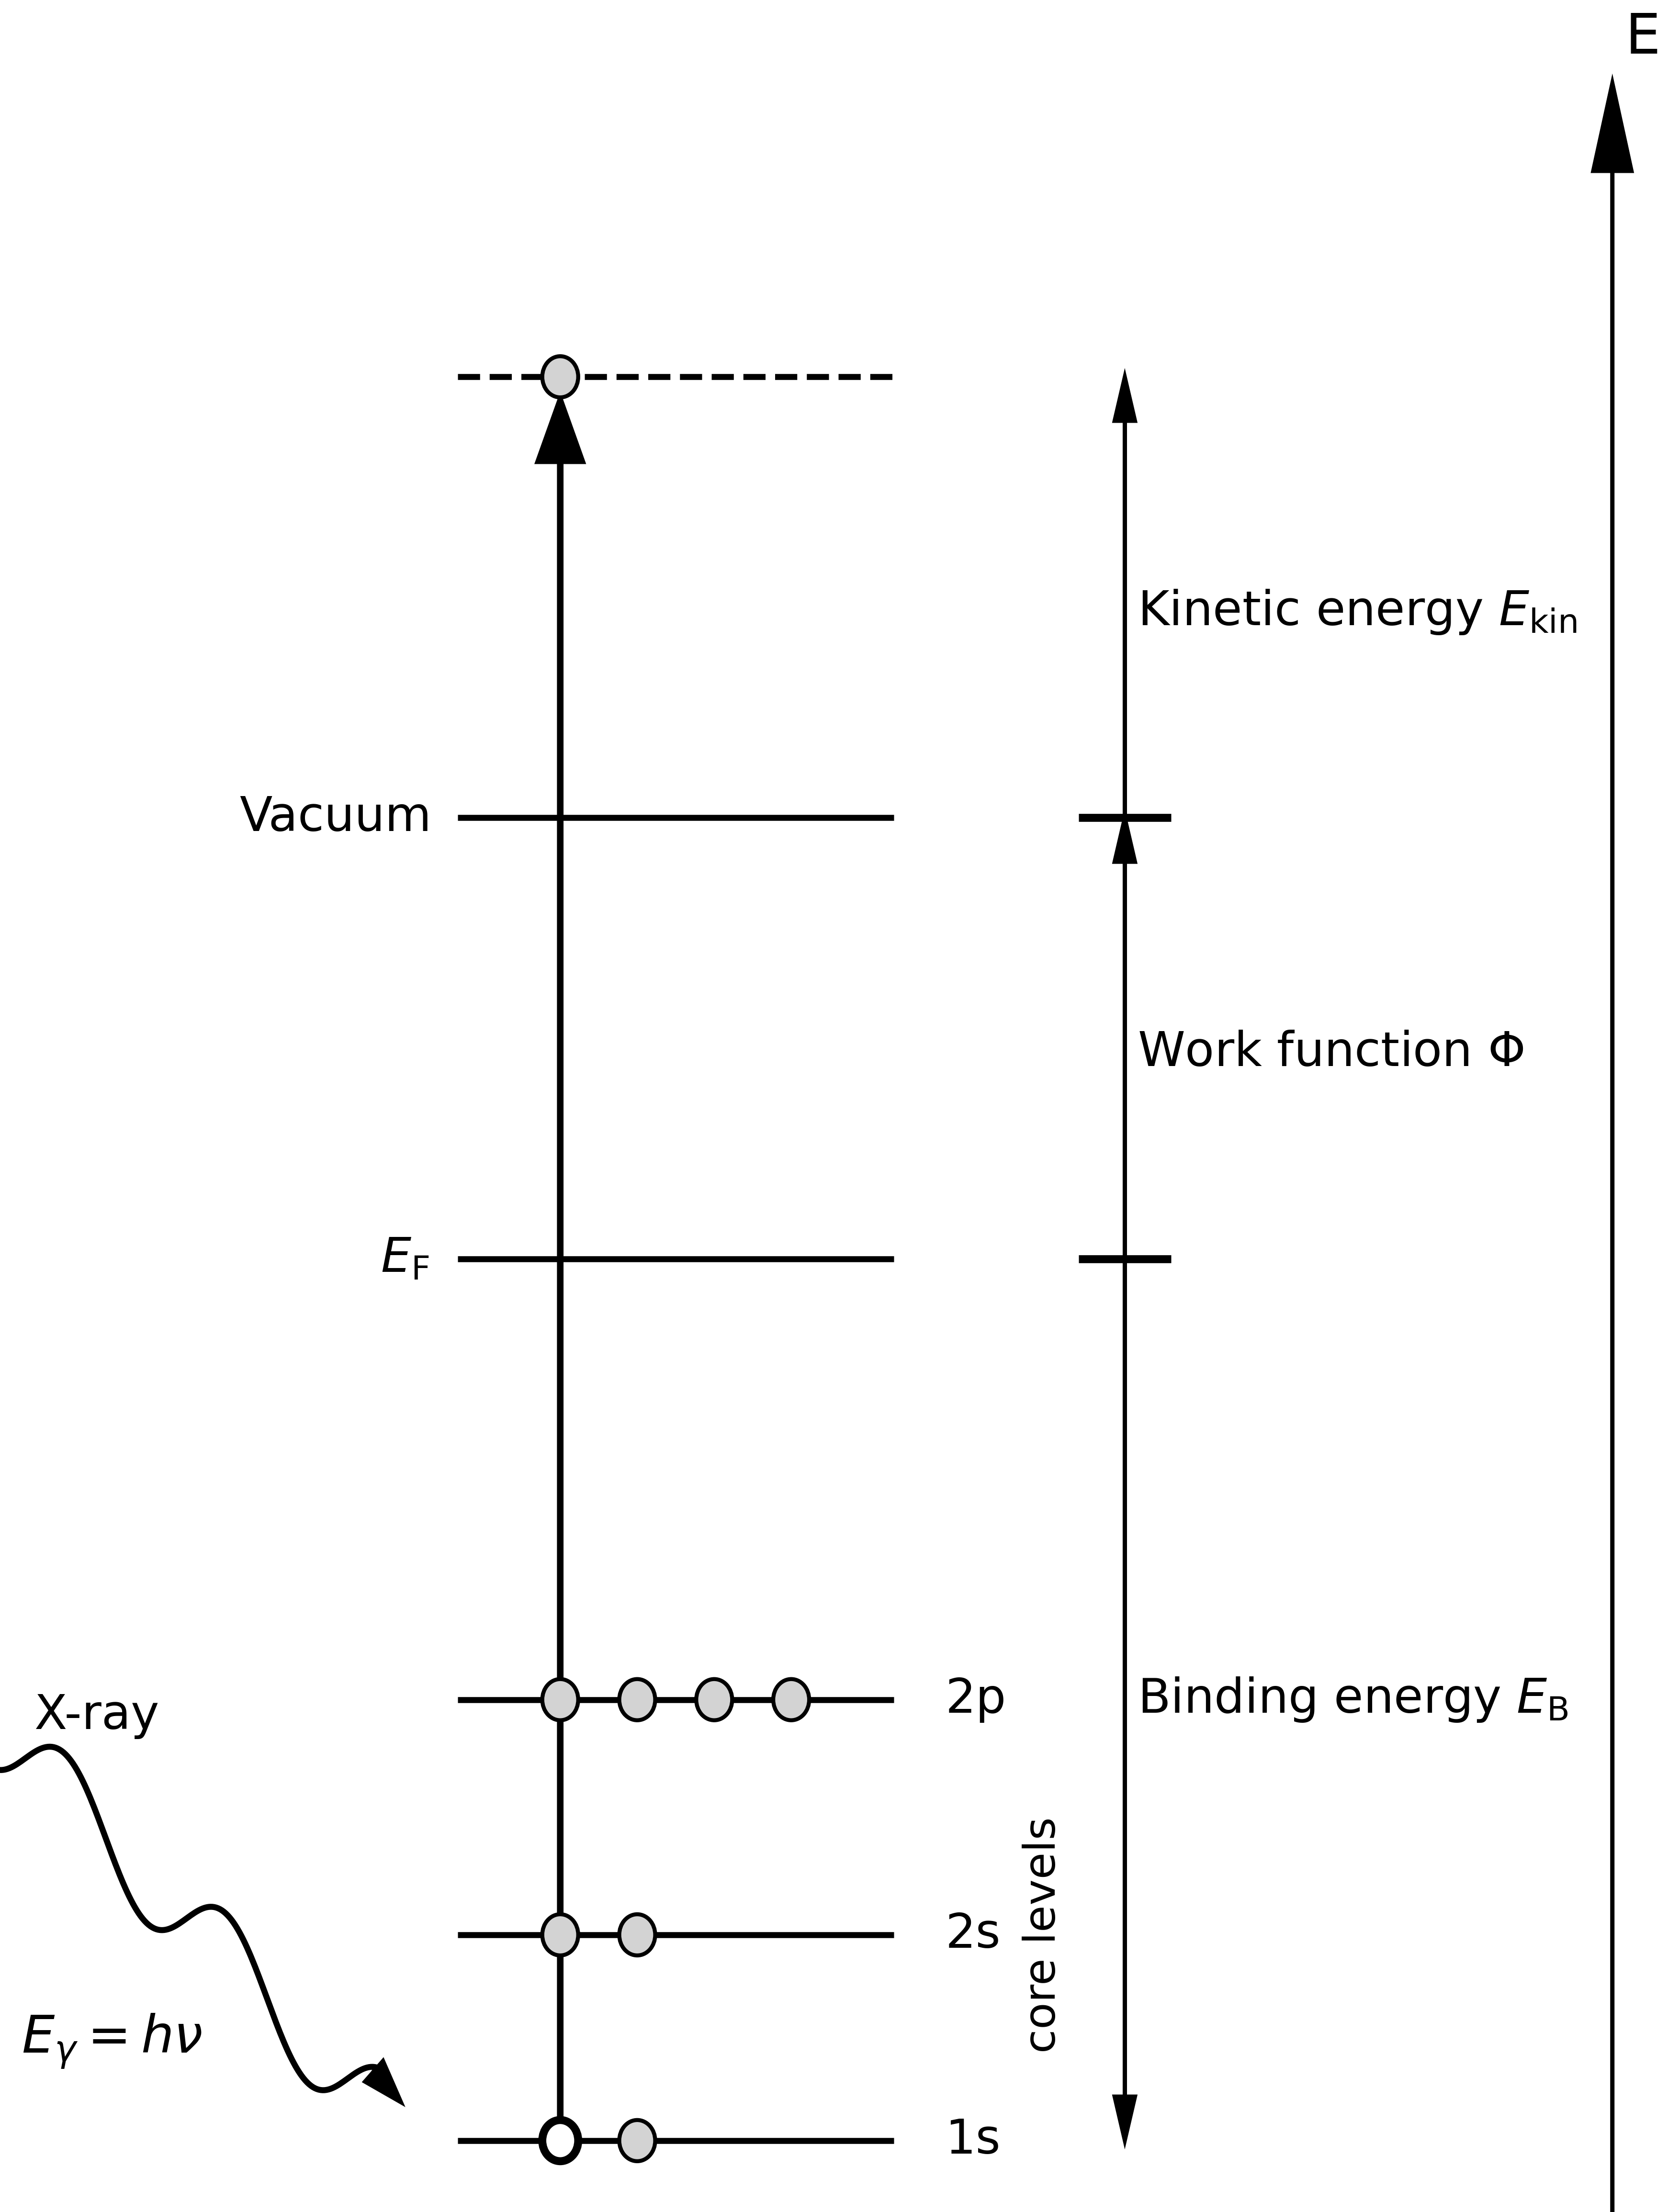
\includegraphics[width=0.48\textwidth]{images/XPS_schematic.png}
	\caption{Schematic drawing of the photoemission process of an electron in the 1s orbital upon x-ray excitation. The image has been illustrated using reference \cite{Attard1998}.}
	\label{fig:XPS-schematic}
\end{figure}

The kinetic energy of the photoelectron $E_\mathrm{kin}$, that is referenced against the Fermi level $E_\mathrm{F}$ for solid substrates by convention, is given by\autocite{Woodruff2016,Briggs1992}:

\begin{equation}
    \label{eq:KineticEnergy1}
    E_\mathrm{kin} = E_\mathrm{\gamma} - E_\mathrm{B},
\end{equation}

where $E_\mathrm{B}$ denotes the \acl{BE} of the photoelectron. Without referencing against $E_\mathrm{F}$, one would also take the work function of the sample $\phi_\mathrm{sample}$ into account:

\begin{equation}
	\label{eq:KineticEnergy2}
	E_\mathrm{kin} = E_\mathrm{\gamma} - E_\mathrm{B}-\phi_\mathrm{sample}.
\end{equation}

 $E_\mathrm{B}$ of an electron is defined as the difference in energies between the atom with $n$ electrons and the ion with $n-1$ electrons:

\begin{equation}
    \label{eq:BindingEnergy}
    E_\mathrm{B}=E_\mathrm{f}(n-1)-E_\mathrm{i}(n)~,
\end{equation}

As seen in this equation, the \ac{BE} of photoelectrons depends on initial and final state effects. The initial state effects manifest for the neutral unexcited atom, due to its interaction with its immediate electronic environment, also referred to as the chemical environment. In addition, final state effects emerge from the correlation between the photoemission process and the ionized final state. The rapid nature of the photoemission process may preclude the system from attaining adiabatic equilibrium.\autocite{Woodruff2016}

The final state effects are characterized by the presence of satellites with reduced kinetic energy, correlating to increased \ac{BE}. This is exemplified by phenomena such as shake-up lines or asymmetric line shapes of the signal, which are indicative of photoemission from the metal surface. The asymmetric line shapes result from coupling of the photoelectrons to the conduction electrons.\autocite{Moulder1993}
A multitude of factors have been identified as contributors to the line shape, particulary the \ac{FWHM}, of the photoemission lines. These include phonon broadening, the lifetime of the photohole, the spectral resolution of the exciting x-ray beam and the energy resolution of the analyzer.\autocite{Moulder1993,Fairley2021}

\cleardoublepage